\section{Module 2: Lecture 2\\Sinusoidal Input to LSI Systems}


\subsection{Introduction}
In this lecture we will learn how to deal with phase changes in sinusoidal signals and pass sinusoidal signals into stable LSI systems in an intelligent and insightful manner. We will look into why we introduced complex signals in our previous analysis and how these tools make the mathematical modelling simple. We then go on to understanding how to deal with signals beyond the domain of sinusoids.


\subsection{Understanding Phase Change In Sinusoids and Phasors}
If we consider a sinusoid as a combination of two rotating complex numbers, which we will henceforth call phasors, moving in opposite direction, 
\[
	2Acos(\Omega t + \phi) = Ae^{j(\Omega t + \phi)} + Ae^{-j(\Omega t + \phi)}
\]
Let us focus our attention on one of the phasors for now. Let us look at what happens when we introduce a phase change.\\
\[
Ae^{j(\Omega t + \phi)} \xrightarrow{Phase \ Change} Ae^{j(\Omega t + \phi + \Delta\phi)}
\]
\[
Ae^{j(\Omega t + \phi + \Delta\phi)} =
Ae^{j(\Omega t + \phi)}e^{j\Delta\phi}
\]
We hence find that a change of phase results just in a multiplying factor which is a constant independent of time.\\
Now we try to do a similar calculation for the complex conjugate (the phasor moving in the opposite direction).
\[
Ae^{-j(\Omega t + \phi)} \xrightarrow{Phase \ Change} Ae^{-j(\Omega t + \phi)}e^{-j\Delta\phi}
\]
Notice that it is the complex conjugate of the previous multiplying factor we found.\\
\[
	2Acos(\Omega t + \phi) \xrightarrow{Phase \ Change} Ae^{j(\Omega t + \phi)}e^{j\Delta\phi} + Ae^{-j(\Omega t + \phi)}e^{-j\Delta\phi}
\]
We hence understand that using only one phasor is enough to fully determine the behaviour of the sinusoid. This explains why we used complex signals in our previous analysis, due to their ease in mathematical understanding.\\
We will now see the result of inputting a sinusoidal signal to a stable linear shift invariant system, with impulse response h(t) (Assume that the impulse response is real).\\
We deal with stable LSI because what we can say from the stability of the system is that y(t) is going to be bounded.\\
\begin{figure}[h!]
\begin{center}
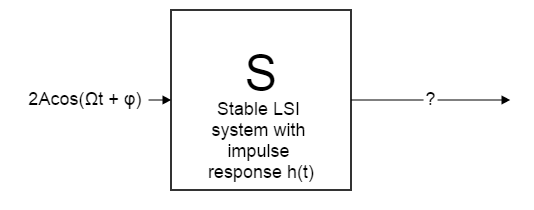
\includegraphics[width=10cm]{LSIcos.png}
\caption{Sinusoidal Input To Stable LSI System}
\end{center}
\end{figure}\\
The direct solution via convolution seems very difficult. In fact if you try to calculate via the convolution integral, we get the following expression.
\[
y(t) = \int_{-\infty}^{+\infty}{h(\lambda)2Acos(\Omega(t-\lambda) + \phi)d\lambda}\]
We will now see how to solve it using phasors, making the analysis mathematically convenient.

  
\subsection{Phasor Input to LSI System}
Consider the output when a phasor is input into a Stable LSI system.

\[
Ae^{j(\Omega t + \phi)} \xrightarrow{LSI} 
 \int_{\infty}^{\infty}Ae^{j(\Omega (t - \lambda + \phi)}h(\lambda)d\lambda
\]
 
\[ =
Ae^{j(\Omega t + \phi)} \int_{\infty}^{\infty}{e^{-j\Omega\lambda}h(\lambda)d\lambda}
\]
So, we see that we obtain the input phasor, with a multiplying factor $\int_{-\infty}^{\infty}{e^{-j\Omega\lambda}h(\lambda)d\lambda}$, which is dependent only on $\Omega$ and $h$ (it is constant with respect to time).\\
We will now come back to the importance of why we chose our system to be stable. We will do this by trying to find a bound to the absolute value of the multiplying factor we just found.
\[
| \int_{-\infty}^{\infty}{e^{-j\Omega\lambda}h(\lambda)d\lambda} | \leq 
\int_{-\infty}^{\infty} { |e^{-j\Omega\lambda}||h(\lambda)| d\lambda }
\]
\[
\int_{-\infty}^{\infty} { |e^{-j\Omega\lambda}||h(\lambda)| d\lambda } =
\int_{-\infty}^{\infty} {|h(\lambda)| d\lambda }
\]
And as per the condition of stability the integral of the absolute value of the impulse response is bounded. Hence the absolute value of the multiplying factor is also bounded. In fact we have obtained a concrete bound to this integral, namely the absolute integral of the impulse response. We can do similar mathematical analysis for the conjugate as well.\\
This multiplying factor is called the \textit{Frequency Response} of the LSI system at angular frequency $\Omega$.
\[
	Frequency\ Response\ H(\Omega) = \int_{-\infty}^{\infty}{e^{-j\Omega\lambda}h(\lambda)d\lambda}
\] 


\subsection{Sinusoid Input to LSI System}

We will now come back to our original problem of inputting a sinusoidal signal into a stable linear shift invariant system. We'll begin by simplifying the outputs of the two phasors.
\[
	H(\Omega)Ae^{j(\Omega t + \phi)} = |H(\Omega)|Ae^{j(\Omega t + \phi +  \angle  H(\Omega))}
\]
The complex conjugate of the frequency response is given by
\[
\bar{H}(\Omega) = \int_{-\infty}^{\infty}{e^{j\Omega\lambda}h(\lambda)d\lambda} = H(-\Omega)
\]
Hence,
\[
H(-\Omega)Ae^{-j(\Omega t + \phi)} = |H(\Omega)|Ae^{-j(\Omega t + \phi +  \angle  H(\Omega))}
\]
Hence by the formula for summing conjugate complex numbers, the output for inputting a sinusoid given by $2Acos(\Omega t + \phi)$ is given by:

\[
2Acos(\Omega t + \phi) \xrightarrow{Stable\ LSI} 2A|H(\Omega)|cos(\Omega t + \phi + \angle H(\Omega))
\]
This indicates that on passing through a stable LSI system, a sinusoid goes through an amplitude and phase shift independent of time, and only dependent on the impulse response and angular frequency of the sinusoid.\\
Also, if we view an input to a stable LSI system as the sum of multiple sinusoids, the output can be visualized as the sum of the corresponding outputs of the sinusoids through the stable LSI system. The stability of the LSI systems guarantees the existence of the frequency response of the system. But if it is unstable it may or may not have a frequency response.


\subsection{Periodic Input to Shift Invariant Systems}
Periodic inputs can be represented by a linear combination (which can be countably infinite) of sinusoids having frequencies which are multiples of the frequency of the input. This property is referred to as a Fourier Series expansion of the input. \\
The Fourier Series expansion and our understanding from the previous section gives us a simple method to compute the output of a periodic input in an LSI system as the linear combination of the output of these sinusoids.\\
First consider the following lemma.\\
\textbf{Lemma:} A periodic input to a shift invariant system produces a periodic output.\\
\textbf{Proof:}\\

Let input x(t) with period T
\[x(t+T) = x(t)\ \ \forall t\]
\[x(t) \xrightarrow{SI\ system} y(t) \]

Now by shift invariance
\[x(t+T) \xrightarrow{SI\ system} y(t+T) \]
\[y(t) = y(t+T)\ \ \forall t \]
Hence the output is also periodic, infact with the same period T.


\subsection{Conclusion}
In this lecture we understood the analysis of inputting sinusoidal input to a stable LSI system. We saw how we could simplify our analysis by the use of phasors. In the upcoming lecture we will learn about the use of inner product and vector analysis in understanding signals.

